\documentclass[a4paper,11pt]{article}
\usepackage[T1]{fontenc}
\usepackage[utf8]{inputenc}
\usepackage{lmodern}
\usepackage{xcolor}
\usepackage[margin=1in]{geometry}
\usepackage{graphicx}
\usepackage{caption}
\usepackage{subcaption}
\usepackage{float}
\usepackage[french]{babel}
\usepackage{listings}
\usepackage{tabularx}
\graphicspath{ {./images/} }
\definecolor{codegreen}{rgb}{0,0.6,0}
\definecolor{codegray}{rgb}{0.5,0.5,0.5}
\definecolor{codepurple}{rgb}{0.58,0,0.82}
\definecolor{backcolour}{rgb}{0.95,0.95,0.92}

\lstdefinestyle{mystyle}{
    backgroundcolor=\color{backcolour},   
    commentstyle=\color{codegreen},
    keywordstyle=\color{magenta},
    numberstyle=\tiny\color{codegray},
    stringstyle=\color{codepurple},
    basicstyle=\ttfamily\footnotesize,
    breakatwhitespace=false,         
    breaklines=true,                 
    captionpos=b,                    
    keepspaces=true,                 
    numbers=left,                    
    numbersep=5pt,                  
    showspaces=false,                
    showstringspaces=false,
    showtabs=false,                  
    tabsize=2
}
\lstset{style=mystyle}

\title{TIPE - La ville}
\author{Valentin FOULON}

\begin{document}
\date{2021-2022}

\maketitle
\tableofcontents


\section{Introduction}
\subsection{Mots-clés}
\begin{tabularx}{0.9\textwidth} { 
  | >{\centering\arraybackslash}X 
  | >{\centering\arraybackslash}X | 
  }
 \hline
 \textbf{Français} & \textbf{Anglais} \\ 
 \hline
 Problème de plus court chemin & Shortest path problem \\ 
 \hline
 Pavage triangulaire / hexagonal & Triangular / hexagonal tiling \\ 
 \hline
 Apprentissage automatique & Machine learning \\ 
 \hline
 Migration pendulaire (déplacement maison - travail) & Commuting \\ 
 \hline
 Optimisation & Optimization \\ 
 \hline
\end{tabularx}

\subsection{Problématique}
Comment créer une infrastructure de transports publics dans une ville afin de minimiser l’attente tout en respectant certaines conditions ?

\subsection{Résumé}
L’objet de ce TIPE est de partir d’une ville dans laquelle il n’y a aucune ligne de transport public, et à partir des points d’affluence de cette ville, les créer de la façon idéale, c’est-à-dire en permettant de transporter le plus de passagers possible, le plus rapidement possible, tout en respectant des conditions de distance d’accès au transport le plus proche, de fiabilité/sécurité, etc. Ici, l’exemple utilisé sera celui du métro, qui ne possède pas de contrainte de direction car il faut créer entièrement sa trajectoire. De plus, il est idéal de prévoir un 

\subsection{Motivation}
Venant de la banlieue parisienne éloignée, j'ai remarqué que l'accès à Paris est difficile par les transports en commun (RER). En effet, les deux lignes principales pour rejoindre la capitale sont souvent problématiques, il y a toujours un incident, que ce soit des travaux sur les lignes en plein milieu de l'été, des bagages abandonnés, etc. J'ai donc voulu chercher des solutions à ce problème.

\subsection{Lien avec la ville}
Les villes tendent à s’agrandir avec le temps, ce qui nécessite des moyens de transport autre que la marche. Mais de plus en plus de villes réduisent la circulation des voitures, en réduisant leur vitesse (par exemple à Paris), en supprimant des voies, ou encore en créant des espaces entièrement piétons (c’est le cas de Dijon). Il faut donc pour cela proposer des moyens de déplacement alternatifs. Malheureusement, toutes les villes ne sont pas égales pour permettre à ses habitants de se déplacer. En particulier, les banlieues sont souvent laissées de côté et les temps de déplacement sont très élevés. Ce TIPE s’inscrit donc dans le thème de la ville.

\section{Sous-problèmes}
\subsection{Distance entre les stations}
La distance entre deux stations joue énormément dans le temps de déplacement. Il faut d’un côté rapprocher les stations afin que les passagers n’aient pas à marcher trop longtemps ni à faire de grandes distances pour se déplacer. Mais il faut également garder une distance suffisante entre deux stations. En effet, un métro doit faire des arrêts pour laisser monter et descendre et monter des passagers. Multiplier les arrêts implique de s’arrêter plus souvent, mais aussi avoir une vitesse moyenne inférieure, et enfin d’avoir moins de rames sur une même ligne.

Prenons deux lignes (1) et (2). La ligne (1) possède deux stations aux extrémités et la ligne (2) possède une station au milieu en plus. Sur chacune des deux lignes, cinq trains de 1000 passagers sont placés. En supposant que les stations ont une affluence infinie, que la vitesse des trains sur une ligne est constante et que les trains de la ligne (1) déposent 1000 passagers à chaque station et ceux de la ligne (2) déposent 500 passagers à chaque station, on obtient le résultat suivant :

pour que chaque ligne transporte le même nombre de passagers en un temps donné, il faut donc que les trains de la ligne (1) mettent le même temps que ceux de la ligne (2) pour aller d’une extrémité à l’autre . Cependant, dans des conditions réelles, les trains doivent accélérer et ralentir autour des stations. Si on rallonge la durée de trajet sur la ligne (2) de 10\% pour prendre en compte les ralentissements, alors la ligne (1) transporte 12,5\% de voyageurs de plus que la ligne (2).

\begin{figure}[H]
\centering
  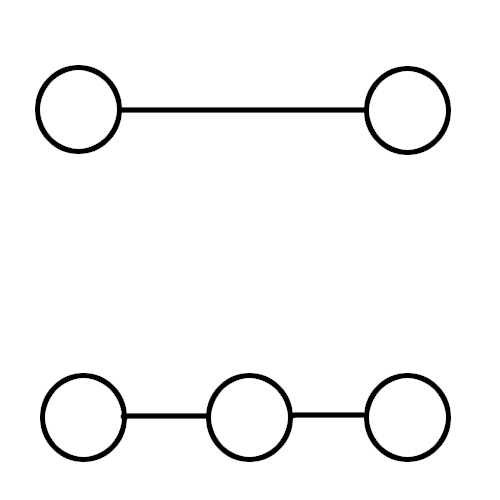
\includegraphics[width=0.4\textwidth]{lignes}
    \caption{Ligne (1) en bas et (2) en haut}
\end{figure}

Pour limiter que les passagers marchent trop, l'idéal est donc d'avoir plusieurs stations de lignes différentes autour d'une même zone. Pour s'assurer de ne jamais dépasser cette distance, il est possible de créer les stations sur un maillage triangulaire ou hexagonal, ce qui permet d'être sûr que la distance maximale d pour rejoindre une station quelconque à partir de toute position est majorée.
Dans les deux cas : soit un triangle équilatéral ou un hexagone de côté a. On a :
\begin{displaymath}
  d \leq \frac{1}{2} \sqrt {a^2 - \left(\frac{a}{2}\right)^2}
\end{displaymath}

\begin{figure}[H]
     \centering
     \begin{subfigure}[b]{0.4\textwidth}
         \centering
         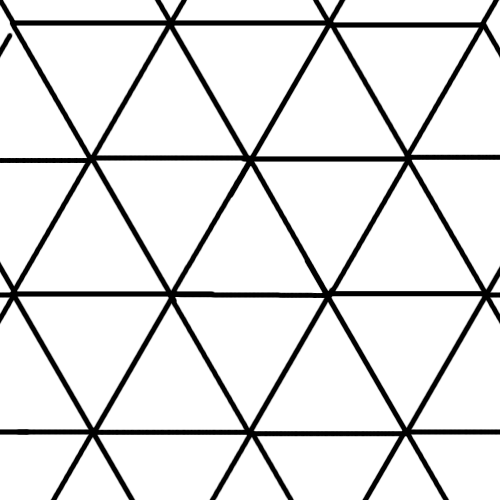
\includegraphics[width=\textwidth]{tri}
         \caption{Pavage triangulaire}
     \end{subfigure}
     \hfill
     \begin{subfigure}[b]{0.4\textwidth}
         \centering
         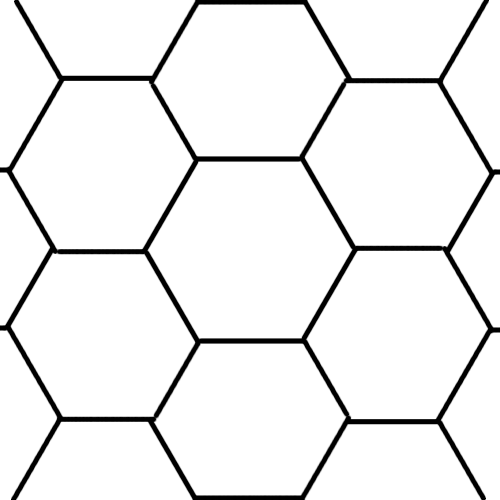
\includegraphics[width=\textwidth]{hex}
         \caption{Pavage hexagonal}
     \end{subfigure}
        \caption{Pavages possibles}
\end{figure}

Hypothèse : laisser une distance maximale de 500m pour aller à n'importe quelle station

\textbf{\textit{A vérifier}}

\subsection{Espacement entre les trains}
L’espacement entre les rames est aussi un facteur à prendre en compte. Il faut réussir à s’adapter à l’affluence des lignes, c’est-à-dire savoir combien de voyageurs sont attendus à un certain moment. Les heures de départ et de retour du travail nécessitent par exemple d’avoir plus de rames en circulation, de même pour les vacances, etc. Mais le nombre de rames sur une ligne est limité. En effet, il faut pouvoir arrêter les autres rames à temps pour éviter des accidents, et éviter de faire attendre un train juste avant une station pour attendre que le précédent parte. De plus, avoir plus de rames sur une ligne augmente le risque d’incidents. Or pour éviter d’avoir une attente importante après l’incident, en général toute la ligne est mise en pause pour conserver un écart égal entre tous les trains.

\textbf{\textit{A exploîter}}


\subsection{Information aux voyageurs}
Un autre élément très important est l’information aux voyageurs. Aujourd’hui, tout le monde possède un téléphone portable ainsi qu’un forfait de téléphone avec un accès à Internet. Grâce aux téléphones, il est possible d’améliorer encore les trajets des voyageurs. Par exemple, en centralisant tout sur une application mobile utilisant du machine learning, il serait possible de réduire considérablement les temps d’attentes:
\begin{itemize}
  \item En permettant aux usagers de prévoir leur titre de transport, alors on peut réduire les files d'attente aux guichets, faire payer les usagers exactement ce qu'ils doivent payer en sachant leur point de départ et leur destination
  \item En leur proposant un itinéraire le plus adapté en fonction des prochains départs, du temps de trajet total (avec un algorithme de plus court chemin, possiblement de Dijkstra), du temps de correspondance (si il y en a une), et de l'affluence à l'heure du trajet
  \item Les deux points précédents réunis ont un autre avantage : limiter l'attente pendant les heures de pointe. En effet, si l'application sait quel sera la destination de l'usager, elle peut aussi prendre en compte l'affluence, et suggérer un itinéraire alternatif qui sera peut-être légèrement plus long, mais permettra aux usagers qui prennent le même chemin tous les jours puissent avoir un trajet de même durée que d'habitude
\end{itemize}

Algorithmes de plus court chemin à envisager :
\begin{itemize}
  \item Dijkstra (O(|E| + |V|log|V|)) : \begin{math} d_{ij} = min_k(d_{ij}, d_{ik} + w(k, j)) \end{math}
  \item Bellman-Ford (O(|V||E|)) : pour u et v voisins \begin{math} d[v] = min(d[v], d[u] + w(u, v)) \end{math}
  \item Floyd-Warshall (O(|V|3)) : \begin{math} \delta(i, j) = min_k(\delta(i, j), \delta(i, k) + \delta(k, j)) \end{math}
\end{itemize}

\textbf{\textit{A exploîter}}

\subsection{Agrandissement}
Lorsqu'une ville vient à s'agrandir dans une direction, il faut relier cette nouvelle partie au reste de la ville. Pour cela, deux solutions majeures sont envisageables :
\begin{itemize}
  \item Agrandir une ligne existante
  \item Créer une nouvelle ligne
\end{itemize}

\textbf{\textit{A exploîter}}

\subsection{Autres idées à explorer}
\begin{itemize}
  \item L'impact des virages d'angle inférieur à 90° sur la vitesse d'un train
  \item Le potentiel gain de temps des trains autonomes
  \item L'impact de la longueur des rames
  \item Possibilité de "synchroniser" l'arrivée des rames dans une station pour les correspondances (soit en les faisant arriver en même temps soit en les alternant)
\end{itemize}



\section{Sources}
A compléter

\section{Code}
\subsection{metro.c (incomplet)}
\begin{figure}[H]
\centering
  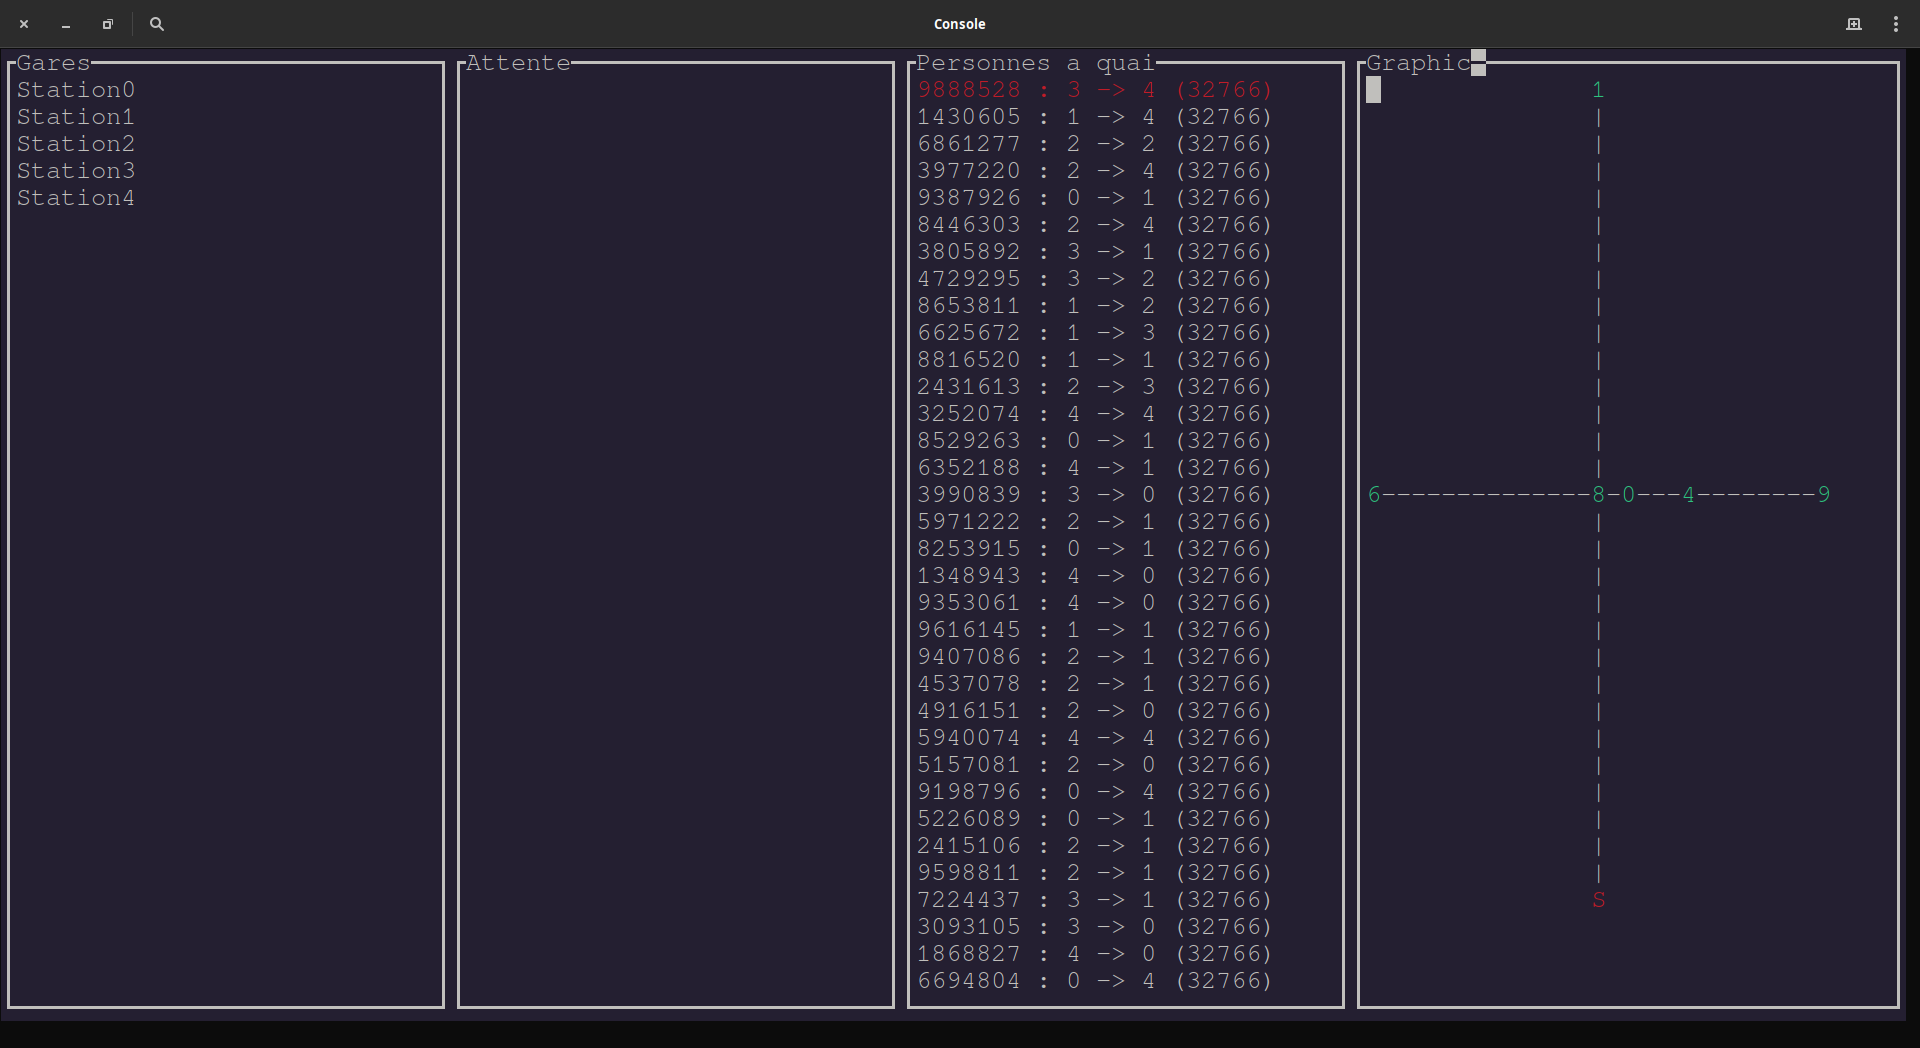
\includegraphics[width=\textwidth]{metro_c}
    \caption{L'interface graphique du programme (pas encore finie)}
\end{figure}

\lstinputlisting[language=C]{metro.c} 
\subsection{vector.h (nécessaire pour le code précédent)}
\lstinputlisting[language=C]{vector.h}

\end{document}
